\documentclass[fin1, tisk, bibtex]{fmfdelo}
% Če pobrišete možnost tisk, bodo povezave obarvane,
% na začetku pa ne bo praznih strani po naslovu, …

%%%%%%%%%%%%%%%%%%%%%%%%%%%%%%%%%%%%%%%%%%%%%%%%%%%%%%%%%%%%%%%%%%%%%%%%%%%%%%%
% METAPODATKI
%%%%%%%%%%%%%%%%%%%%%%%%%%%%%%%%%%%%%%%%%%%%%%%%%%%%%%%%%%%%%%%%%%%%%%%%%%%%%%%

% - vaše ime
\avtor{Jon Pascal Miklavčič}

% - naslov dela v slovenščini
\naslov{Weierstrass-Enneperjeva konstrukcija minimalnih ploskev}

% - naslov dela v angleščini
\title{Weierstrass-Enneper construction of minimal surfaces}

% - ime mentorja/mentorice s polnim nazivom:
%   - doc.~dr.~Ime Priimek
%   - izr.~prof.~dr.~Ime Priimek
%   - prof.~dr.~Ime Priimek
%   za druge variante uporabite ustrezne ukaze
\mentor{doc.~dr.~Uroš Kuzman}
% \somentor{...}
% \mentorica{...}
% \somentorica{...}
% \mentorja{...}{...}
% \somentorja{...}{...}
% \mentorici{...}{...}
% \somentorici{...}{...}

% - leto diplome
\letnica{2026} 

% - povzetek v slovenščini
%   V povzetku na kratko opišite vsebinske rezultate dela. Sem ne sodi razlaga
%   organizacije dela, torej v katerem razdelku je kaj, pač pa le opis vsebine.
\povzetek{
    V diplomskem delu obravnavamo minimalne ploskve v evklidskih prostorih $\mathbb{R}^3$. Lokalno jih opišemo kot grafe, ki zadoščajo Euler--Lagrangeovi enačbi ploščinskega funkcionala, kar je ekvivalentno pogoju, da je njihova srednja ukrivljenost enaka nič. Kompleksna analiza pokaže, da je konformna imerzija iz odprte ravninske domene $D \subseteq \mathbb{C}$ v Evklidski prostor minimalna ploskev natanko tedaj, ko je harmonična. Ta rezultat omogoča reprezentacijo minimalnih ploskev s parom holomorfne in meromorfne funkcije na $D$ preko Weierstrass-Enneperjeve formule. Izreke ponazorimo s klasičnimi primeri minimalnih ploskev: katenoido, helikoidom in Enneperjevo ploskvijo. 
}

% - povzetek v angleščini
\abstract{
    In this thesis, we study minimal surfaces in Euclidean space $\mathbb{R}^3$. We describe them locally as graphs satisfying the Euler--Lagrange equation of the area functional, which is equivalent to the condition that their mean curvature is zero. Complex analysis reveals that a conformal immersion from an open planar domain $D \subseteq \mathbb{C}$ into a Euclidean space is a minimal surface if and only if it is harmonic. This result enables the representation of minimal surfaces by a pair of a holomorphic and a meromorphic function on $D$ via the Weierstrass-Enneper formula. We illustrate the theorems with classical examples of minimal surfaces: the catenoid, the helicoid, and Enneper's surface.
}

% - klasifikacijske oznake, ločene z vejicami
%   Oznake, ki opisujejo področje dela, so dostopne na strani https://www.ams.org/msc/
\klasifikacija{53A10, 49Q05, 53C42, 58E12}

% - ključne besede, ki nastopajo v delu, ločene s \sep
\kljucnebesede{minimalna ploskev\sep variacijski račun\sep Weierstrass-Enneperjeva reprezentacija\sep konformna harmonična preslikava}

% - angleški prevod ključnih besed
\keywords{minimal surface\sep calculus of variations\sep Weierstrass-Enneper representation\sep conformal harmonic map} % angleški prevod ključnih besed

% - angleško-slovenski slovar strokovnih izrazov
\slovar{
    \geslo{area functional}{ploščinski funkcional}
    \geslo{catenary}{verižnica}
    \geslo{catenoid}{katenoida}
    \geslo{conformal map}{konformna preslikava}
    \geslo{Enneper's surface}{Enneperjeva ploskev}
    \geslo{helicoid}{helikoid}
    \geslo{holomorphic function}{holomorfna funkcija}
    \geslo{isothermal coordinates}{izotermne koordinate}
    \geslo{mean curvature}{srednja ukrivljenost}
    \geslo{meromorphic function}{meromorfna funkcija}
    \geslo{minimal surface}{minimalna ploskev}
    \geslo{principal curvatures}{glavni ukrivljenosti}
    \geslo{ruled surface}{premonosna ploskev}
    \geslo{surface of revolution}{rotacijska ploskev}
    \geslo{Weierstrass-Enneper representation}{Weierstrass-Enneperjeva reprezentacija}
}
% \geslo{angleški izraz}{slovenski izraz}



% - ime datoteke z viri (vključno s končnico .bib), če uporabljate BibTeX
\literatura{literatura.bib}

%%%%%%%%%%%%%%%%%%%%%%%%%%%%%%%%%%%%%%%%%%%%%%%%%%%%%%%%%%%%%%%%%%%%%%%%%%%%%%%
% DODATNE DEFINICIJE
%%%%%%%%%%%%%%%%%%%%%%%%%%%%%%%%%%%%%%%%%%%%%%%%%%%%%%%%%%%%%%%%%%%%%%%%%%%%%%%

% naložite dodatne pakete, ki jih potrebujete
\usepackage{tikz}
\usepackage{pgfplots}
\usepackage{subcaption}
\usepackage[scr=rsfs]{mathalpha}

% tikz 
\pgfplotsset{compat=1.18}
%\newcommand{\samplescalar}{5}  % hitro compilanje
\newcommand{\samplescalar}{50} % high-res

% deklarirajte vse matematične operatorje, da jih bo LaTeX pravilno stavil
% \DeclareMathOperator{\...}{...}

% vstavite svoje definicije ...
% \newcommand{\...}{...}

%%%%%%%%%%%%%%%%%%%%%%%%%%%%%%%%%%%%%%%%%%%%%%%%%%%%%%%%%%%%%%%%%%%%%%%%%%%%%%%
% ZAČETEK VSEBINE
%%%%%%%%%%%%%%%%%%%%%%%%%%%%%%%%%%%%%%%%%%%%%%%%%%%%%%%%%%%%%%%%%%%%%%%%%%%%%%%

\begin{document}

\section{Uvod}

Minimalne ploskve so gladke ploskve v prostoru, ki lokalno minimizirajo ploščino v smislu, da ima vsak dovolj majhen del ploskve najmanjšo ploščino med vsemi ploskvami z istim robom. Ta lastnost jih tesno povezuje z zakoni fizike. Naraven primer je milni mehurček, napet na žičnato ogrodje, ki zavzame obliko minimalne ploskve. Zaradi prisotnosti v vsakdanjem življenju in še zaradi številnih drugih lepih geometrijskih lastnosti so že pred več stoletji pritegnile pozornost.

Teorija minimalnih ploskev ima bogato zgodovino. Z njimi so se ukvarjali skoraj vsi vidnejši matematiki 19.~in 20.~stoletja. Prvi je o problemu, ki ga danes poznamo pod imenom \glqq minimalne ploskve\grqq{} razmišljal Joseph-Louis Lagrange okoli leta 1768, ko si je zamislil naslednji variacijski problem: najti ploskev z najmanjšo površino, ki jo omejuje dana sklenjena krivulja. Lagrange je ta problem prevedel na iskanje stacionarnih točk ploščinskega funkcionala in izpeljal t.~i.~enačbo za minimalne grafe, ki jo mora (lokalno) izpolnjevati vsaka minimalna ploskev. Lagrange netrivialne rešitve te enačbe ni odkril.  Po slabem desetletju je leta 1776 Jean Baptiste Meusnier kot rešitvi Euler--Lagrangeove variacijske enačbe našel helikoid, ki je bil poleg katenoide takrat edina znana netrivialna minimalna ploskev. Poleg tega pa je prišel še do naslednjega pomembnega spoznanja: ploskve z ničelno srednjo ukrivljenostjo so natanko tiste, ki minimizirajo ploščino v Lagrangeovem smislu~\cite{enciklopedia}. 

Že v tem kratkem uvodu smo naleteli na tri ekvivalentne, a povsem drugačne definicije minimalne ploskve. A kljub temu je poiskati parametrizacijo minimalne ploskve izjemno zahtevno. Tudi preverjanje, ali je dana ploskev res minimalna, je pogosto zamudno delo. V 80. letih 19.~stoletja pa sta Karl Weierstrass in Alfred Enneper odkrila način, ki omogoča preprosto konstrukcijo minimalnih ploskev. Njuno delo prikazuje še enega izmed zelo zanimivih vidikov minimalnih ploskev. Ležijo na presečišču več na prvi pogled nepovezanih področij matematike. Že iz uvoda je mogoče razbrati, da združujejo diferencialno geometrijo, variacijski račun in kompleksno analizo.

Diplomska naloga se bo posvetila zgoraj omenjeni Weierstrass-Enneperjevi reprezentaciji minimalnih ploskev. Temelji na uporabi kompleksnih analitičnih funkcij, kar omogoča ne samo boljše razumevanje teh objektov, ampak tudi enostavno konstrukcijo primerov minimalnih ploskev.

\newpage




\section{Ukrivljenost}

\subsection{Ukrivljenost krivulj}
Preden začnemo obravnavati minimalne ploskve, si moramo najprej natančneje ogledati koncepta ukrivljenosti krivulj in ploskev. Začnimo s krivuljami.

\begin{definicija}
    Pravimo, da je afina preslikava $\mathbb{R}^n \rightarrow \mathbb{R}^n$ oblike $x \mapsto A x+b$ \emph{toga}, če je $b \in \mathbb{R}^n$ in $A\in \mathbb{R}^{n\times n}$ ortogonalna matrika (t.~j.~$A^T A = I$).
\end{definicija}

Privzamemo lahko, da se krivljenost krivulje ali ploskve ne spremeni pod togo preslikavo.

Pri izpeljavi ukrivljenosti ploskev v naslednjem razdelku bomo videli, da zadošča, da si na tem mestu ogledamo koncept ukrivljenosti le za ravninske krivulje $\gamma \subseteq\mathbb{R}^2$. Na krivulji izberemo poljubno točko $p \in \gamma$ in jo s togim premikom premaknemo v koordinatno izhodišče, njeno tangento $T_p \gamma$ pa na os $x$. Kot omenjeno zgoraj, s tem ukrivljenosti krivulje nismo spremenili. Če se skličemo še na izrek o implicitni funkciji, lahko na to krivuljo v okolici točke $(0,0)$ gledamo kot na graf funkcije $y=f(x)$. Očitno velja $f(0)=f^{\prime}(0)=0$. 

\begin{trditev}
    Naj bo $f$ dvakrat zvezno odvedljiva funkcija. Ukrivljenost grafa $f$ v točki $x$ je
    \begin{equation*}
        \kappa(x)=\frac{f^{\prime \prime}(x)}{\left(1+\left(f^{\prime}(x)\right)^2\right)^{3/2}}.
    \end{equation*}
\end{trditev}

Dokaz trditve najdemo~\cite[str.~156]{ana2}. Ker v našem primeru velja $f^{\prime}(0)=0$, se bo potem iskana ukrivljenost glasila
\begin{equation}
    \kappa=f^{\prime \prime}(0). \label{eq:ukrivljenost}
\end{equation}
Imenujemo jo \emph{predznačena ukrivljenost} krivulje v točki $(0,0)$. Njeno absolutno vrednost $|\kappa|=\left|f^{\prime \prime}(0)\right| \geq 0$ pa \emph{ukrivljenost}.


\subsection{Ukrivljenost ploskev}

Nadaljujmo zdaj z ukrivljenostjo ploskev. Natančneje, pogledali si bomo koncepta glavnih ukrivljenosti in srednje ukrivljenosti gladke ploskve v prostoru $\mathbb{R}^3$. Pri tem bomo sledili~\cite[Razdelek 3]{fosternicmin}.

Naj bo $S \subseteq \mathbb{R}^3$ gladka ploskev. Naj bodo $(x, y, z)$ koordinate v $\mathbb{R}^3$. Na ploskvi fiksiramo točko $p \in S$. S togo spremembo koordinat lahko premaknemo $p$ v $(0,0,0)$ in $T_p S$ v $\mathbb{R}^2 \times\{0\}$. Potem lahko, tako kot prej, $S$ okoli koordinatnega izhodišča izrazimo kot graf oblike $z=f(x, y)$. Izberemo si zdaj enotski vektor $v=\left(v_1, v_2\right)$ v ravnini $(x,y)$. S $\Sigma_v$ označimo ravnino skozi koordinatno izhodišče, ki jo razpenjata vektor $v$ in koordinatna os $z$. Presečišče $\gamma_v:=S \cap \Sigma_v$ je krivulja na $S$ podana kot
\begin{equation*}
    z=f\left(v_1 t, v_2 t\right)
\end{equation*}
za $t \in \mathbb{R}$ blizu $0$. Iz prejšnjega razdelka o ukrivljenosti krivulj in dobljene formule (\ref{eq:ukrivljenost}) vemo, da je $\kappa_v=\left.\frac{\mathrm{d}^2}{\mathrm{d} t^2}\right|_{t=0} f\left(v_1 t, v_2 t\right)$ predznačena ukrivljenost krivulje $\gamma_v$ v točki $(0,0)$. Če poračunamo drugi odvod funkcije $f$, po uporabi verižnega pravila dobimo
\begin{align}
    \frac{\mathrm{d}}{\mathrm{d} t}f\left(v_1 t, v_2 t\right) &= f_x\left(v_1 t, v_2 t\right) v_1 + f_y\left(v_1 t, v_2 t\right) v_2 \notag \\
    \frac{\mathrm{d}^2}{\mathrm{d} t^2}f\left(v_1 t, v_2 t\right) &= v_1\left(f_{x x} v_1 + f_{x y} v_2\right) + v_2\left(f_{y x} v_1 + f_{y y} v_2\right) \notag \\
    &= f_{x x} v_1^2 + 2 f_{x y} v_1 v_2 + f_{y y} v_2^2 \label{eq:drugi_odvod}
\end{align}
Če se spomnimo še definicije Hessejeve matrike funkcije $f$ v točki $(0,0)$ 
\begin{equation}
    A=\begin{bmatrix}
        f_{x x}(0,0) & f_{x y}(0,0) \\
        f_{x y}(0,0) & f_{y y}(0,0)
    \end{bmatrix} \label{eq:hessejeva}
\end{equation}
lahko enačbo (\ref{eq:drugi_odvod}) zapišemo v obliki kvadratne forme $\kappa_v= A v \cdot v$. Na enotski krožnici $|v|^2=v_1^2+v_2^2=1$ kvadratna forma $v \mapsto A v \cdot v$ kot zvezna funkcija na kompaktni množici doseže svoj \emph{maksimum} $\kappa_1$ in \emph{minimum} $\kappa_2$.

\begin{figure}[ht]
    \centering
    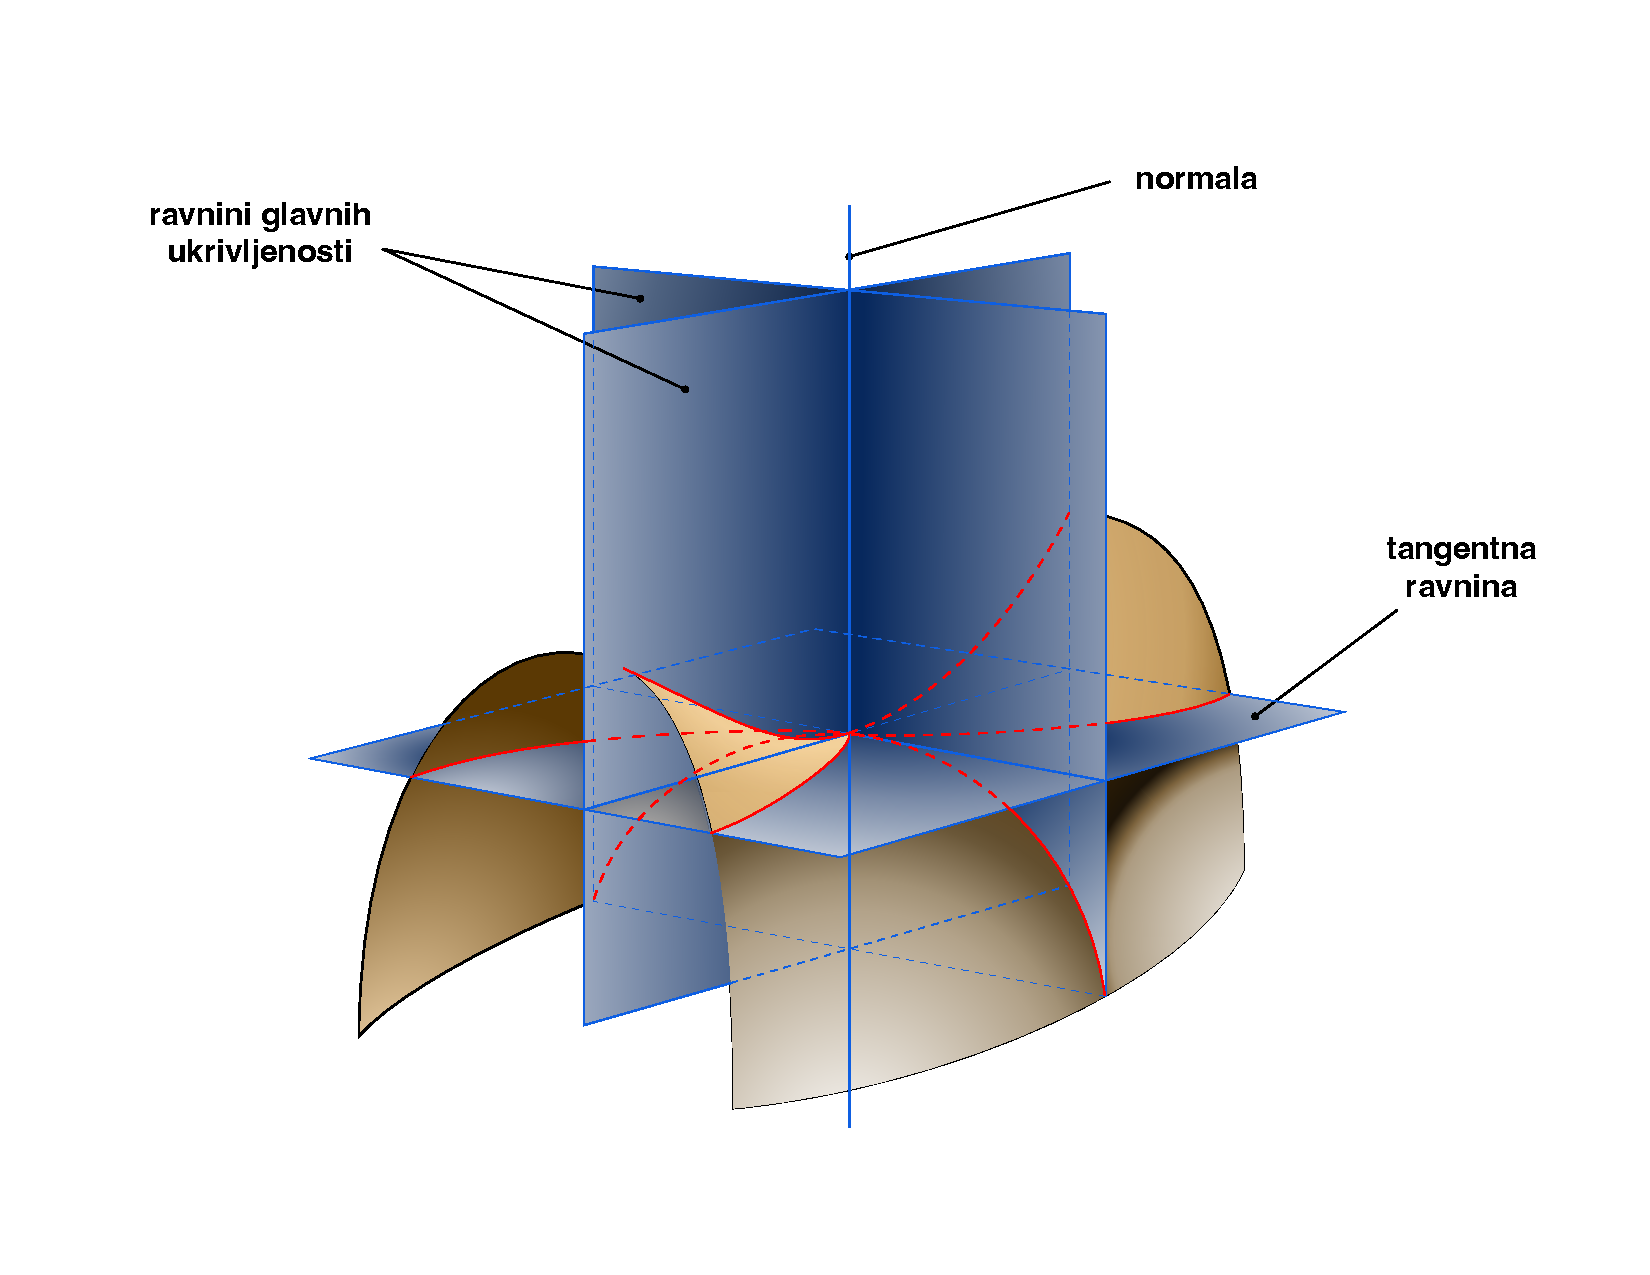
\includegraphics[width=20em]{../Slike/Minimal_surface_curvature_planes_slo.pdf}
    \caption{Konstrukcija za izračun srednje ukrivljenosti~\cite{wiki}.}
\end{figure}

\begin{definicija}
    Vrednosti $\kappa_1$ in $\kappa_2$ iz zgornje izpeljave imenujemo \emph{glavni ukrivljenosti} ploskve $S$ v točki $(0,0,0)$. 
\end{definicija} 
Ker je matrika $A$ simetrična, sta $\kappa_1$ in $\kappa_2$ njeni lastni vrednosti.
\begin{definicija}
    \emph{Srednja ukrivljenost} ploskve $S$ v $(0,0, 0)$ je
    \begin{equation*}
        H=\frac{1}{2}(\kappa_1+\kappa_2)=\frac{1}{2}\operatorname{sled} (A)
    \end{equation*}
\end{definicija} 
Tukaj je vredno pripomniti še, da je sled matrike $A$ (\ref{eq:hessejeva}) enaka $\Delta f(0,0)=f_{x x}(0,0)+f_{y y}(0,0)$, kjer je $\Delta$ Laplaceov operator. Po drugi strani pa je sled matrike enaka vsoti njenih lastnih vrednosti. To implicira 
\begin{equation}
    \Delta f(0,0)=\kappa_1+\kappa_2=2H \label{eq:Laplace_H}.
\end{equation}




\section{Minimalne ploskve}

Sedaj pa se lahko posvetimo minimalnim ploskvam. Kot omenjeno v uvodu, je grobo rečeno minimalna ploskev taka, ki lokalno minimizira ploščino. Da dobimo boljšo predstavo, kako pridemo do takih ploskev, si bomo najprej ogledali izpeljavo enačbe minimalnih grafov kot Euler--Lagrangeovo enačbo ploščinskega funkcionala. Če na neko funkcijo, katere graf je minimalna ploskev, gledamo kot na funkcijo, ki minimizira ploščinski funkcional -- to je gladko preslikavo iz prostora funkcij v $\mathbb{R}$, ki meri ploščino -- lahko z uporabo metod variacijskega računa pokažemo, da je minimiziranje ploščine ekvivalentno temu, da je srednja ukrivljenost ploskve povsod enaka nič.


\subsection{Grafi z minimalno ploščino}

Ogledali si bomo minimalne ploskve v prostoru $\mathbb{R}^3$, predstavili pa jih bomo, vsaj lokalno, kot minimalne grafe. Začnimo z izpeljavo Euler--Lagrangeove enačbe za minimalne grafe (povzeto po~\cite[Razdelek 3.1]{Vrhovnik_2022}). 

Naj bo $D$ omejena podmnožica ravnine $\mathbb{R}^2$ z odsekoma gladkim robom $bD$. Z $\bar{D}$ označimo njeno zaprtje in na njem definiramo funkcijo $f: \bar{D} \rightarrow \mathbb{R}$ razreda $\mathcal{C}^2$. Njen graf je množica
\begin{equation*}
    \Gamma_f=\left\{(x, y, z) \in \mathbb{R}^3 \mid(x, y) \in \bar{D}, z=f(x, y)\right\}
\end{equation*}
njegovo ploščino pa lahko izrazimo s funkcionalom $\mathcal{A}:\mathcal{C}^2(\bar D) \rightarrow \mathbb{R}$:
\begin{equation}
    \mathcal{A}(f)=\iint_{D} \sqrt{1+f_x^2+f_y^2} \, \mathrm{d} x \mathrm{d} y=\iint_{D} \sqrt{1+|\nabla f|^2} \, \mathrm{d} x \mathrm{d} y. \label{eq:area_funkcional}
\end{equation}

Zanimajo nas predvsem funkcije $f$, katerih grafi bodo imeli najmanjšo ploščino med vsemi bližnjimi funkcijami na $\bar{D}$ z enakimi robnimi vrednostmi $\left.f\right|_{b D}: b D \rightarrow \mathbb{R}$. Iščemo torej funkcije s predpisanimi robnimi vrednostmi, ki bodo stacionarne točke ploščinskega funkcionala $\mathcal{A}$ (\ref{eq:area_funkcional}).

Skladno s klasičnimi metodami variacijskega računa bomo pogledali deformacije $f$, ki ne bodo spreminjale robnih vrednosti. Izberemo $\mathcal{C}^1$ funkcijo $h: \bar{D} \rightarrow \mathbb{R}$, za katero velja $h(bD) \equiv 0$, in si ogledamo družino funkcij $\{f+s h | s \in \mathbb{R}\}$. Opazimo, da bo funkcija $f$ stacionarna točka ploščinskega funkcionala $\mathcal{A}$ natanko tedaj, ko bo pri $s=0$ za vse zgoraj opisane deformacije $h$ veljalo 
\begin{equation}
    \left.\frac{\mathrm{d}}{\mathrm{d} s}\right|_{s=0} \mathcal{A}(f+s h)=0. \label{eq:area}
\end{equation}
Pri poenostavljanju enačbe se opremo na naslednjo lemo.
\begin{lema}[Osnovna lema variacijskega računa] \label{lem:variacijski_racuna}
    Če za zvezno funkcijo $f$ na $\bar D \subseteq \mathbb{R}^2$ in za vsako zvezno odvedljivo funkcijo $h$, ki je ničelna na $bD$ velja 
    \begin{equation*}
        \iint_D f(x,y) h(x,y) \, \mathrm{d} x \mathrm{d} y=0,
    \end{equation*}
    potem je $f \equiv 0$ na $\bar D$.
\end{lema}
Enačbo (\ref{eq:area}) poenostavimo. Računamo
\begin{align}
    \left.\frac{\mathrm{d}}{\mathrm{d} s}\right|_{s=0} \mathcal{A}(f+s h) &= \left.\frac{\mathrm{d}}{\mathrm{d} s}\right|_{s=0} \iint_{D} \sqrt{1+\left((f+s h)_x\right)^2+\left((f+s h)_y\right)^2} \, \mathrm{d} x \mathrm{d} y \notag \\
    & =\left.\iint_{D} \frac{\mathrm{d}}{\mathrm{d} s}\right|_{s=0} \sqrt{1+\left(f_x+s h_x\right)^2+\left(f_y+s h_y\right)^2} \, \mathrm{d} x \mathrm{d} y \notag \\
    & =\iint_{D} \frac{f_x h_x+f_y h_y}{\sqrt{1+f_x^2+f_y^2}} \, \mathrm{d} x \mathrm{d} y \notag \\
    & = \iint_{D} \frac{\nabla h \cdot \nabla f}{\sqrt{1+|\nabla f|^2}} \, \mathrm{d} x \mathrm{d} y \label{eq:izracun}
\end{align}
Ker poznamo robne vrednosti deformacije $h$ in funkcije $f$, je na tem koraku  smiselno uporabiti Gaussov izrek~\cite[str.~196]{ana2}, ki nam bo zgornji integral po območju povezal z integralom po robu tega območja. Dokaza izreka ne bomo navajali.
\begin{izrek}[Gaussov izrek]
    Naj bo $D$ omejeno območje v $\mathbb{R}^2$, katerega rob je sestavjen iz končnega števila gladkih krivulj. Orientiramo rob $bD$ tako, da izberemo zunanjo normalo $\mathbf{n}$. Naj bo $\mathbf{F}$ gladko vektorsko polje v okolici $D \cup b D$. Tedaj velja 
    \begin{equation*}
        \iint_{D}\operatorname{div}(\mathbf{F}) \, \mathrm{d}x \mathrm{d}y =\oint_{b D} \mathbf{F} \cdot \mathbf{n} \, \mathrm{d}s .
    \end{equation*}
\end{izrek}
Če ohranimo zapis iz izreka, kjer je $h$ funkcija in $\mathbf{F}$ vektorsko polje ter upoštevamo, da za divergenco velja $\operatorname{div}(h \mathbf{F})=\nabla h \cdot \mathbf{F}+h \cdot \operatorname{div}(\mathbf{F})$, s pomočjo Gaussovega izreka dobimo tako imenovano prvo Greenovo identiteto
\begin{equation*}
    \iint_{D} \nabla h \cdot \mathbf{F} \, \mathrm{d} x \mathrm{d} y=\oint_{b D} h \mathbf{F} \cdot \mathbf{n} \, \mathrm{d} s-\iint_{D} h \, \operatorname{div}(\mathbf{F}) \, \mathrm{d} x \mathrm{d} y.
\end{equation*}
Torej, če v izrazu (\ref{eq:izracun}) izberemo $\mathbf{F}=\frac{\nabla f}{\sqrt{1+|\nabla f|^2}}$, ga lahko nadalje poenostavimo 
\begin{align*}
    \left.\frac{\mathrm{d}}{\mathrm{d} s}\right|_{s=0} \mathcal{A}(f+s h) & =\iint_{D} \nabla h \cdot \frac{\nabla f}{\sqrt{1+|\nabla f|^2}} \, \mathrm{d} x \mathrm{d} y \\
    & =-\iint_{D} h \,\left(\frac{\partial}{\partial x} \frac{f_x}{\sqrt{1+|\nabla f|^2}}+\frac{\partial}{\partial y} \frac{f_y}{\sqrt{1+|\nabla f|^2}}\right) \, \mathrm{d} x \mathrm{d} y,
\end{align*}
kjer smo v drugi enakosti uporabili prvo Greenovo identiteto in upoštevali dejstvo, da je funkcija $h$ na robu $bD$ identično enaka 0. Zaradi zveznosti $h$ -- oziroma po Lemi \ref{lem:variacijski_racuna} -- je izraz enak $0$ za vse izbore $h$ natanko takrat, ko na domeni $D$ velja 
\begin{equation*}
    \frac{\partial}{\partial x} \frac{f_x}{\sqrt{1+|\nabla f|^2}}+\frac{\partial}{\partial y} \frac{f_y}{\sqrt{1+|\nabla f|^2}}=0.
\end{equation*}   
Zgornjo enačbo lahko poenostavimo in dobimo:
\begin{align*}
    \frac{\partial}{\partial x} \frac{f_x}{\sqrt{1+f_x^2+f_y^2}}+\frac{\partial}{\partial y} \frac{f_y}{\sqrt{1+f_x^2+f_y^2}} & =\frac{f_{x x}\left(1+f_x^2+f_y^2\right)-f_x\left(f_x f_{x x}+f_y f_{x y}\right)}{\left(1+f_x^2+f_y^2\right)^{3 / 2}} \\
    & \qquad +\frac{f_{y y}\left(1+f_x^2+f_y^2\right)-f_y\left(f_x f_{x y}+f_y f_{y y}\right)}{\left(1+f_x^2+f_y^2\right)^{3 / 2}} \\
    & =\frac{f_{x x}\left(1+f_y^2\right)-2 f_x f_y f_{x y}+f_{y y}\left(1+f_x^2\right)}{\left(1+f_x^2+f_y^2\right)^{3 / 2}}.
\end{align*}
Na tem mestu definiramo že prej omenjeno enačbo za minimalne grafe.

\begin{definicija}
    Eliptično kvazilinearno parcialno diferencialno enačbo drugega reda imenujemo \emph{enačba za minimalne grafe}
    \begin{equation}
        \left(1+f_y^2\right) f_{x x}-2 f_x f_y f_{x y}+\left(1+f_x^2\right) f_{y y}=0. \label{eq:min_enacba}
    \end{equation}
\end{definicija}

Ta enačba je ekvivalentna enačbi (\ref{eq:area}). Naravno vprašanje, ki se porodi na tem mestu, je vprašanje o obstoju reštve te parcialne diferencialne enačbe pri zvezno določenih robnih vrednostih na $bD$ in o njeni enoličnosti. Ta Dirichletov problem za enačbo minimalnega grafa je leta 1930 razrešil T. Radó, in sicer za omejena konveksna območja.

\begin{trditev}
    Naj bo $D \subseteq \mathbb{R}^2$ omejena konveksna množica z robom $bD$ in $g$ zvezna funkcija, definirana na $bD$. Potem obstaja rešitev enačbe minimalnih grafov \emph{(\ref{eq:min_enacba})}, t.~j.~funkcija $f$, definirana na $D$, ki zavzame enake robne vrednosti kot $g$.     
\end{trditev}

Dokaz trditve najdemo v~\cite[str.~61]{osserman2002survey}. Iz principa za maksimalne grafe pa sledi, da je rešitev enolična. Iz izpeljave enačbe za minimalne grafe vemo, da funkcija, ki minimizira ploščino glede na dane robne vrednosti zadošča enačbi za minimalne grafe. Omenimo, da velja tudi obratna trditev. 
\begin{trditev}\label{thm:min_ploskev_1}
    Če funkcija $f\in \mathcal{C}^2(D)$, definirana na konveksni domeni $D\subseteq \mathbb{R}^2$ zadošča enačbi za minimalne grafe, potem $f$ minimizira ploščino glede na dane robne vrednosti. 
\end{trditev}
Dokaz trditve najdemo v~\cite[str.~69]{morgan2016geometric}. Zgornja trditev nam zagotavlja, da dovolj majhni delčki minimalne ploskve res minimizirajo ploščino. To pa ne velja nujno za večje dele ploskve -- protiprimer je lahko že Enneperjeva ploskev. Del Enneperjeve ploskve prikazan na sliki (\ref{fig:enneperjeva_min_a}) ne minimizira ploščine glede na njen rob. Ploskvi z istim robom, ki minimizirata ploščino, sta prikazani na sliki (\ref{fig:enneperjeva_min_b}).
\begin{figure}[htbp]
    \centering
    \begin{subfigure}{0.45\textwidth}
        \centering
        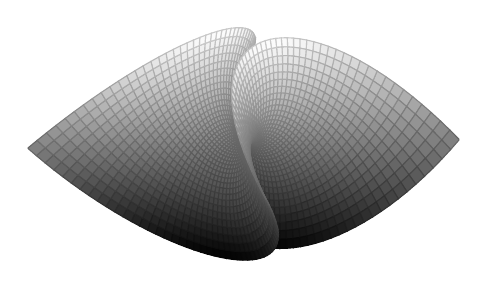
\begin{tikzpicture}
            \begin{axis}[
                view={220}{15},
                samples=\samplescalar, 
                samples y=\samplescalar,
                domain=-1.3:1.3, 
                y domain=-1.3:1.3,
                scale=0.8,
                axis lines=none,
                colormap={bw}{gray(0cm)=(0); gray(1cm)=(1)},
            ]
            
            % Enneperjeva ploskev 
            \addplot3[
                surf,
                z buffer = sort,
            ]
            (
                {x - (1/3) * x^3 + x * y^2}, 
                {-y - x^2 * y + (1/3) * y^3}, 
                {x^2 - y^2} 
            );

            \end{axis}
        \end{tikzpicture}
        \caption{\small Enneperjeva ploskev}
        \vspace{1.15em}
        \label{fig:enneperjeva_min_a}
    \end{subfigure}\hfill
    \begin{subfigure}{0.45\textwidth}
        \centering
        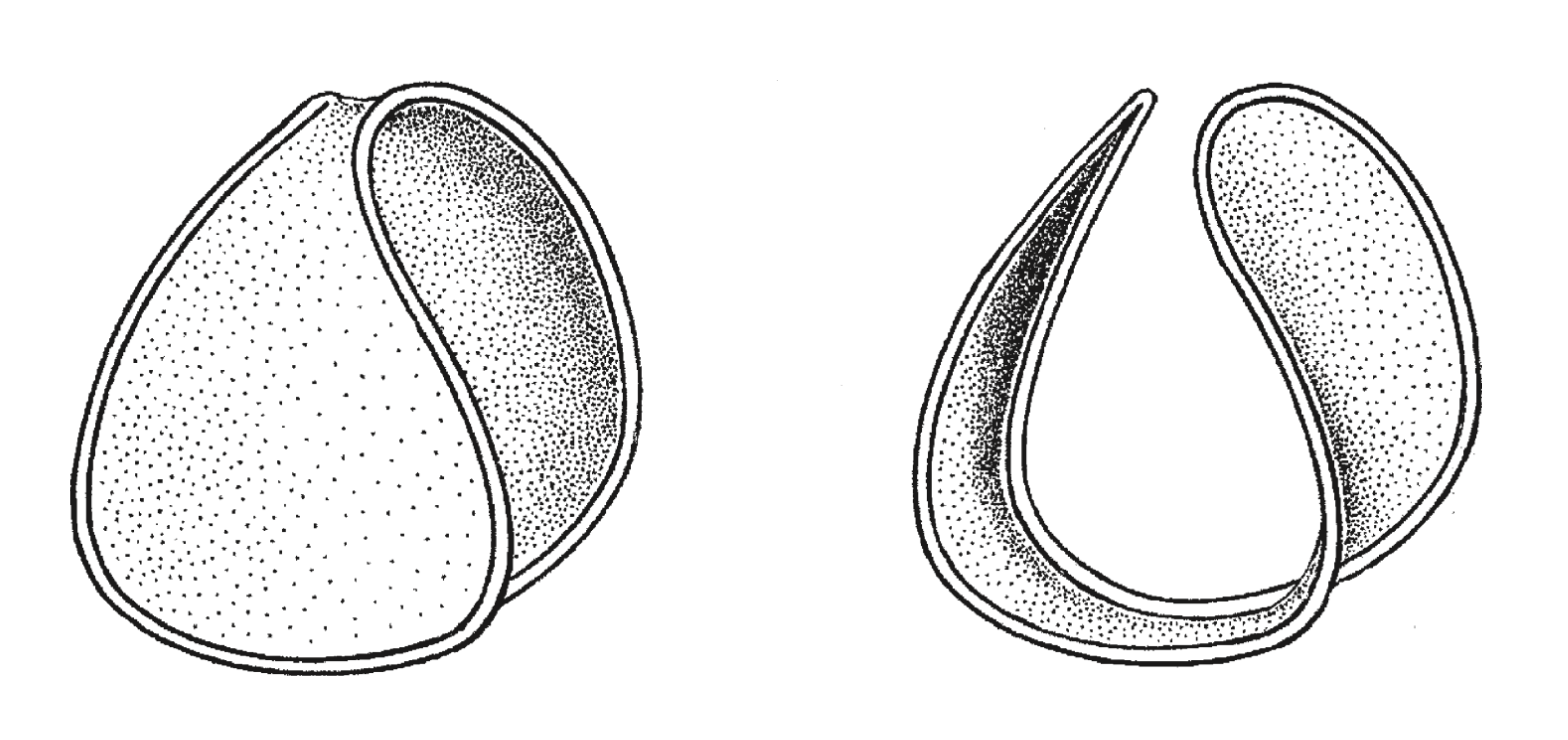
\includegraphics[width=16em]{../Slike/enneper_global_minimization_counterexample}
        \caption{\small Ploskvi z minimalno ploščino in enakim robom kot Enneperjeva ploskev~\cite{morgan2016geometric}.}
        \label{fig:enneperjeva_min_b}
    \end{subfigure}
    \caption{Minimalna ploskev minimizira površino samo lokalno.}
\end{figure}

\begin{opomba}
    Že v uvodu smo omenili, da je \glqq biti minimalen\grqq{} lokalna lastnost. S pomočjo zgornjega razmisleka lahko to definiramo natančneje.
    Če poljubna točka $\left(x_0, y_0\right) \in D$ premore odprto okolico $U \subseteq D$ z lastnostjo, da za vsako zvezno odvedljivo funkcijo $h_U$, ki je ničelna izven množice $U$ velja $\left.\frac{\mathrm{d}}{\mathrm{d} s}\right|_{s=0} \mathcal{A}\left(f+s h_U\right)=0$, potem funkcija $f$ reši enačbo za minimalne grafe (\ref{eq:min_enacba}). Zaključimo, da je graf minimalen natanko tedaj, ko je minimalen v okolici vsake točke~\cite[str.~16]{Vrhovnik_2022}.
\end{opomba}


\subsection{Karakterizacija s srednjo ukrivljenostjo}

Na tem koraku bomo geometrijsko interpretirali enačbo za minimalne grafe (\ref{eq:min_enacba}). Naslednjo trditev je leta 1776 dokazal Meusnier in s tem karakteriziral minimalne grafe z ukrivljenostjo. 

\begin{trditev} \label{thm:srednja_ukrivljenost}
    Funkcija $f: D \rightarrow \mathbb{R}$ razreda $\mathcal{C}^2$, definirana na domeni $D \subseteq \mathbb{R}^2$, reši enačbo za minimalne grafe 
    \begin{equation}
        \mathcal{G}(f):=\left(1+f_y^2\right) f_{x x}-2 f_x f_y f_{x y}+\left(1+f_x^2\right) f_{y y}=0 \label{eq:trvitev1}
    \end{equation}
    natanko tedaj, ko ima njen graf $\Gamma_f$ v vsaki točki  ničelno srednjo ukrivljenost. 
\end{trditev}

Ta trditev nam pove, da je vsaka točka na minimalni ploskvi sedlo, kar pomeni, da se ploskev krivi enako močno, a v nasprotnih smereh v obeh glavnih smereh. Poglejmo si zdaj dokaz te trditve (povzet po~\cite[str.~6]{fosternicmin}).

\begin{dokaz}
    Izberimo poljubno točko $\left(x_0, y_0\right) \in D$. Ker sta enačba za minimalne grafe in srednja ukrivljenost $H$ invarianti glede na toge premike v $\mathbb{R}^3$, lahko z ustrezno translacijo in rotacijo okoli osi $z$ brez škode za splošnost privzamemo, da je $\left(x_0, y_0\right)=(0,0), f(0,0)=0$ ter $\nabla f(0,0)=(a, 0)$ za nek $a \geq 0$. Morda bi si želeli doseči $a=0$, vendar taka rotacija ne bi nujno ohranila lastnosti, da je $f$ graf nad ravnino $(x,y)$. Ekvivalenco torej dokazujemo v koordinatnem izhodišču. 
    
    Izberimo naslednjo ortonormirano bazo $\mathbb{R}^3$:
    \begin{equation*}
        \mathbf{v}_1=\frac{1}{\sqrt{1+a^2}}(1,0, a), \quad \mathbf{v}_2=(0,1,0), \quad \mathbf{v}_3=\frac{1}{\sqrt{1+a^2}}(-a, 0,1).
    \end{equation*}
    Vidimo, da $\mathbf{v}_1$ in $\mathbf{v}_2$ razpenjata tangentno ravnino $T_0 S$ v $(0,0)$, $\mathbf{v}_3$ pa je njena normala. Označimo z $(u, v, w)$ koordinate, ki so vezane na to bazo. Torej se prvotne koordinate izrazijo kot 
    \begin{equation*}
        (x, y, z)=u \mathbf{v}_1+v \mathbf{v}_2+w \mathbf{v}_3.
    \end{equation*}
    Po izreku o implicitni funkciji lahko v koordinatah $(u,v,w)$ plosev $S$ na okolici koordinatnega izhodišča podamo kot graf oblike
    \begin{equation*}
        w=g(u, v), \quad g(0,0)=0, \quad \nabla g(0,0)=(0,0).
    \end{equation*}
    Tako kot prej bo srednja ukrivljenost $S$ v točki $(0,0)$ enaka $H=\frac{1}{2}\Delta g(0,0)$. Za dokončanje dokaza bomo $\mathcal{G}(f)(0,0)$ izrazili z $\Delta g(0,0)$. V koordinatah $(x, y, z)$ je ploskev $S$ parametrizirana kot 
    \begin{equation*}
        x=\frac{1}{\sqrt{1+a^2}}(u-a g(u, v)), \quad y=v, \quad z=\frac{1}{\sqrt{1+a^2}}(a u+g(u, v)) .
    \end{equation*}
    Ker je $S$ prav tako podana z $z=f(x, y)$, dobimo izraz
    \begin{equation*}
        a u+g(u, v)=\sqrt{1+a^2} \cdot f\left(\frac{u-a g(u, v)}{\sqrt{1+a^2}}, v\right) .
    \end{equation*}
    Enačbo dvakrat implicitno odvajamo po $u$ in po $v$
    \begin{align*}
        g_u & =f_x\left(1-a g_u\right) - a\\
        g_v & =f_x\left(-a g_v\right)+f_y \sqrt{1+a^2} \\
        g_{u u} & =\frac{f_{x x}\left(1-a g_u\right)^2}{\sqrt{1+a^2}}+f_x\left(-a g_{u u}\right) \\
        g_{v v} & =\frac{f_{x x}\left(-a g_v\right)^2}{\sqrt{1+a^2}}+f_x\left(-a g_{v v}\right)+f_{x y}\left(-2 a g_v\right)+f_{y y} \sqrt{1+a^2} .
    \end{align*}
    Če druge parcialne odvode ovrednotimo pri $(u, v)=(0,0)$, kar se ujema z $(x, y)=(0,0)$, in upoštevamo $f_x(0,0)=a, f_y(0,0)=0, g_u(0,0)=g_v(0,0)=0$, dobimo 
    \begin{align*}
        g_{u u}(0,0) & =\frac{f_{x x}(0,0)}{\sqrt{1+a^2}}-a^2 g_{u u}(0,0) \\
        g_{v v}(0,0) & =-a^2 g_{v v}(0,0)+f_{y y}(0,0) \sqrt{1+a^2}
    \end{align*}
    in tako 
    \begin{equation*}
        f_{x x}(0,0)={\sqrt{1+a^2}}^3 g_{u u}(0,0), \quad f_{y y}(0,0)=\sqrt{1+a^2} g_{v v}(0,0).
    \end{equation*}
    Tako v $(0,0)$ dobimo
    \begin{align*}
        \mathcal{G}(f) & =\left(1+f_y^2\right) f_{x x}-2 f_x f_y f_{x y}+\left(1+f_x^2\right) f_{y y} \\
        & ={\sqrt{1+a^2}}^3 g_{u u}+\left(1+a^2\right) \sqrt{1+a^2} g_{v v} \\
        & ={\sqrt{1+a^2}}^3 \Delta g .
    \end{align*}
    To pokaže, da velja $\mathcal{G}(f)(0,0)=0$ natanko tedaj, ko je $\Delta g(0,0)=2H=0$.
\end{dokaz}
Trditev \ref{thm:srednja_ukrivljenost} nam pokaže, da ima gladka ploskev v $\mathbb{R}^3$ ničelno srednjo ukrivljenost natanko tedaj, ko je v vsaki svoji točki $p_0 \in S$ minimalni graf nad pripadajočo tangentno ravnino $T_{p_0} S$. S tem smo dobili novo karakterizacijo minimalnih ploskev.

\begin{opomba}
    Tako kot definicija minimalne ploskve kot lokalne rešitve enačbe za minimalne grafe, je tudi definicija s pomočjo srednje ukrivljenosti lokalna. 
    
    %V obeh primerih smo na ploskev v okolici vsake točke gledali kot na sliko ravninske domene. Kljub temu da je veliko klasičnih primerov minimalnih ploskev, kot so katenoida, helikoid in Enneperjeva ploskev, parametriziranih z ravninskimi domenami, je globalna struktura minimalne ploskve lahko zelo zapletena in ni nujno slika ravninske domene. 
\end{opomba}




\subsection{Konformna parametrizacija minimalne ploskve}

V tem razdelku bomo spremenili pogled na minimalne ploskve. Na ploskev ne bomo več gledali le eksplicitno kot na graf funkcije, temveč kot na sliko ravninske domene pri gladki preslikavi. Natančneje, obravnavali bomo ploskve, ki so slike \emph{imerzij}. Naj bodo $(u, v)$ koordinate v $\mathbb{R}^2$. 

\begin{definicija}
    Preslikava $F: D \subseteq \mathbb{R}^2 \rightarrow \mathbb{R}^3$ razreda $\mathcal{C}^1$ je \emph{imerzija}, če je njena Jacobijeva matrika
    \begin{equation*}
        JF(u,v) = \begin{bmatrix} \frac{\partial F}{\partial u} & \frac{\partial F}{\partial v} \end{bmatrix} = \begin{bmatrix} F_u & F_v \end{bmatrix} 
    \end{equation*}
    ranga $2$ v vsaki točki $(u,v) \in D$.
\end{definicija}

Zahtevo o maksimalnosti ranga lahko ekvivalentno izrazimo kot zahtevo, da vektorski produkt parcialnih odvodov ni nikoli ničelen:
\begin{equation*}
    F_u \times F_v \neq (0,0,0) \quad \text {za vse }(u, v) \in D .    
\end{equation*}
Slika imerzije $S=F(D) \subseteq\mathbb{R}^3$ predstavlja parametrizirano ploskev. Pogoj, da je vektorski produkt $F_u \times F_v \neq 0$ v vsaki točki neničeln, zagotavlja, da je v vsaki točki ploskve enolično določena tangentna ravnina $T_pS=\operatorname{Lin}\left\{F_u, F_v\right\}$.

%\begin{opomba}
%    Izraz \emph{imerzija} je mogoče bolje poznan pod imenom \emph{regularna parametrizacija}, a je v tem kontekstu bolj smiselna uporabe prve. 
%\end{opomba}

\begin{definicija}
    Imerzija $F: D \rightarrow \mathbb{R}^3$ je \emph{konformna}, če za vsako točko $(u, v) \in D$ veljata naslednja pogoja:
    \begin{equation}
        F_u \cdot F_u=F_v \cdot F_v, \quad F_u \cdot F_v=0. \label{eq:konformnost}
    \end{equation}
\end{definicija}

Če si stvar predstavljamo bolj geometrijsko, je konformna imerzija taka, ki \glqq ohranja kote\grqq{}. To pomeni, da je kot med tangentnima vektorjema poljubnih dveh sekajočih se krivulj v domeni $D$ enak kotu med njunima slikama na ploskvi v $\mathbb{R}^3$.

Preden navedemo in dokažemo naslednjo lemo, se spomnimo, da za diferencibilni vektorski funkciji $f, g: \mathbb{R}^2 \rightarrow \mathbb{R}^3$ velja pravilo za odvod skalarnega produkta:
\begin{equation*}
    (f \cdot g)_u = f_u \cdot g + f \cdot g_u \quad \text{in} \quad (f \cdot g)_v = f_v \cdot g + f \cdot g_v.
\end{equation*}

\begin{lema}\label{lm:laplace}
	Naj bo $D \subseteq \mathbb{R}^2$ in $p \in D$ poljubna točka. Če je $F=\left(x, y, z\right): D \rightarrow \mathbb{R}^3$ konformna imerzija razreda $\mathcal{C}^2$, potem je vektor $\Delta F(p)=\left(\Delta x(p), \Delta y(p), \Delta z(p)\right)$ pravokoten na tangentno ravnino $T_{F(p)}S \subseteq \mathbb{R}^3$. Ekvivalentno,
    \begin{equation}
        \Delta F \cdot F_u =0, \quad \Delta F \cdot F_v = 0 \label{eq:lema_konformnost}
    \end{equation}
    velja povsod na $D$. 
\end{lema}

\begin{dokaz}
    Vemo, da je $F$ konformna. Torej zanjo velja $F_u \cdot F_u=F_v \cdot F_v$ in $F_u \cdot F_v=0$. Prvi pogoj odvajamo po $u$, drugega pa po $v$. Dobljeni enačbi združimo in dobimo  
    \begin{equation*}
        F_{u u} \cdot F_u=F_{u v} \cdot F_v=-F_{v v} \cdot F_u,
    \end{equation*}
    od koder sledi $\left(F_{u u}+F_{v v}\right) \cdot F_u=\Delta F \cdot F_u=0$. Podobno, če potem prvi izraz odvajamo po $v$, drugega pa po $u$, dobimo še $\Delta F \cdot F_v=0$~\cite[str.~8]{fosternicmin}. 
\end{dokaz}

Preden navedemo naslednjo trditev, povejmo še, da je lastnost Laplaceovega operatorja $\Delta F$ v Lemi \ref{lm:laplace} invariantna za toge premike v $\mathbb{R}^n$, ker ohranijo kote. Eksplicitno: za poljubno ortogonalno matriko $A$ dimenzij $n \times n$  in gladko preslikavo $F(u, v)=\left(x_1(u, v), \ldots, x_n(u, v)\right) \in \mathbb{R}^n$, ki slika iz domene v ravnini $D \subseteq\mathbb{R}^2$, velja
\begin{equation}
    \Delta(A \cdot F(u, v))=A \cdot \Delta F(u, v) \label{eq:laplace}
\end{equation}

\begin{trditev} \label{thm:konformna_harmonica_imerzija}
    Konformna imerzija $F=(x, y, z): D \rightarrow \mathbb{R}^3$ razreda $\mathcal{C}^2$, ki slika iz domene $D \subseteq\mathbb{R}^2$ parametrizira ploskev z ničelno srednjo ukrivljenostjo natanko tedaj, ko je $F$ harmonična:
    \begin{equation*}
        \Delta F=(\Delta x, \Delta y, \Delta z)=0
    \end{equation*}
\end{trditev} 
%Še več, konformna imerzija $F: D \rightarrow \mathbb{R}^3$ je harmonična natanko tedaj, ko je stacionarna točka ploščinskega funkcionala. 
\begin{dokaz}
    Izberemo poljubno točko $(u_0,v_0) \in D$. Ker sta tako srednja ukrivljenost kot Laplaceov operator po (\ref{eq:laplace}) invariantna za toge premike, lahko izračun brez škode za splošnost izvedemo v primerno izbranem koordinatnem sistemu. Brez škode za splošnost tako preko translacije predpostavimo $\left(u_0, v_0\right)=(0,0)$. 
    

    Ker je $F$ konformna, zanjo v vsaki točki velja $F_u \cdot F_v=0$ in $\left\|F_u\right\|=\left\|F_v\right\|=\mu>0$. Definiramo še enotsko normalo $\mathbf{N}=\frac{F_u \times F_v}{\left\|F_u \times F_v\right\|}$. Vektorji $\left\{\frac{1}{\mu} F_u, \frac{1}{\mu} F_v, \mathbf{N}\right\}$ tvorijo ortonormirano bazo prostora. Potem vemo, da obstaja ortogonalna matrika, ki te tri bazne vektorje preslika v standardno bazo prostora $\mathbb{R}^3$. Eksplicitno, za $(u, v)=(0,0)$ velja naslednje: 
    \begin{equation}
        x_u=y_v=\mu>0, \quad x_v=y_u=0, \quad z_u=z_v=0, \quad \mathbf{N} = (0,0,1) . \label{eq:odvodi}
    \end{equation}
    Po izreku o implicitni funkciji vemo, da obstaja okolica izhodišča $U \subseteq D$, tako lahko ploskev $S=F(U)$ predstavimo kot graf funkcije $z=f(x, y)$, kjer velja $f_x(0,0)=0$ in $f_y(0,0)=0$.

    Lema \ref{lm:laplace} nam pove, da je $\Delta F$ pravokotna na $(x,y)$ ravnino v koordinatnem izhodišču, kar pomeni, da velja 
    \begin{equation}
        \Delta x(0,0)=\Delta y(0,0)=0. \label{eq:pravokotnost_na_ravnino}
    \end{equation}
    Izračunajmo še $\Delta z(0,0)$. Odvajanje izraza $z(u, v)=f(x(u, v), y(u, v))$ nam da 
    \begin{align*}
        z_u &= f_x x_u + f_y y_u, \\
        z_{uu} &= f_{xx} x_u^2 + 2 f_{xy} x_u y_u + f_{yy} y_u^2 + f_x x_{uu} + f_y y_{uu}, \\[1ex]
        z_v &= f_x x_v + f_y y_v, \\
        z_{vv} &= f_{xx} x_v^2 + 2 f_{xy} x_v y_v + f_{yy} y_v^2 + f_x x_{vv} + f_y y_{vv}.
    \end{align*}
    Upoštevamo (\ref{eq:odvodi}) in $f_x(0,0)=f_y(0,0)=0$. Dobimo $z_{u u}=\mu^2 f_{x x}$ in $z_{v v}=\mu^2 f_{y y}$. Po (\ref{eq:Laplace_H}) vemo, da je srednja ukrivljenost $S$ v točki $0 \in \mathbb{R}^3$ enaka $2H=\Delta f(0,0)$. Iz tega zaključimo, da
    \begin{equation}
        \Delta z(0,0)=\mu^2 \Delta f(0,0)=2\mu^2 H, \label{eq:laplace_z}
    \end{equation}
    Če povzamemo (\ref{eq:odvodi}), (\ref{eq:pravokotnost_na_ravnino}) in (\ref{eq:laplace_z}) dobimo, da
    \begin{equation*}
        \Delta F=2\left|F_u\right|^2 H \mathbf{N}
    \end{equation*}
    velja v $(0,0) \in D$. Specifično, $\Delta F(0,0)=0$ natanko tedaj, ko je $H=0$. Ker ta utemeljitev velja za poljubno točko iz $D$, smo trditev dokazali~\cite[str.8-9]{fosternicmin}. 
\end{dokaz}

Na tem mestu se pojavi naravno vprašanje, ali lahko parametrizacijo poljubne imerzije $F$ vedno zamenjamo s konformno. Odgovor je pritrdilen, vendar le lokalno. Naj bo torej $F: D \rightarrow \mathbb{R}^3$ gladka imerzija. Za vsako točko $p \in D$ obstajata odprta okolica $U \subseteq D$ in tak difeomorfizem (zvezno odvedljiva bijekcija z zvezno odvedljivim inverzom) $\Phi: V \rightarrow U$, $(\tilde{u}, \tilde{v}) \mapsto(u, v)$, da je sestavljena imerzija
\begin{equation*}
    \widetilde{F} = F \circ \Phi : V \rightarrow \mathbb{R}^3
\end{equation*}
konformna. Difeomorfizem $\Phi$ si lahko predstavljamo kot lokalno spremembo koordinat. Tem novim koordinatam $(\tilde{u}, \tilde{v})$ pravimo \emph{izotermne koordinate}. 
To pomeni, da za parcialna odvoda reparametrizirane imerzije $\widetilde{F}$ v novih koordinatah velja:
\begin{equation*}
    \widetilde{F}_{\tilde{u}} \cdot \widetilde{F}_{\tilde{u}}= \widetilde{F}_{\tilde{v}} \cdot \widetilde{F}_{\tilde{v}} \quad \text{in} \quad \widetilde{F}_{\tilde{u}} \cdot \widetilde{F}_{\tilde{v}} = 0.
\end{equation*}

Obstoj izotermnih koordinat je za rotacijske ploskve dokazal C.~F.~Gauss. Dokaz v splošnem primeru je prezahteven in ga ne navajamo. Najdemo ga lahko v~\cite[Razdelek 1.8]{monograf}.




\section{Minimalne ploskve skozi kompleksno analizo}

V tem razdelku se bomo posvetili Weierstrass-Enneperjevi reprezentaciji, ki vzpostavlja neposredno povezavo med holomorfnimi preslikavami $D \rightarrow \mathbb{C}^3$ s posebnimi lastnostmi, kjer je $D \subseteq \mathbb{C}$ ravninska domena, in konformnimi minimalnimi imerzijami $D \rightarrow \mathbb{R}^3$. Za začetek si poglejmo nekaj osnovnih pojmov in ključnih rezultatov iz kompleksne analize, ki jih bomo potrebovali v nadaljevanju.


\subsection{Kompleksna analiza}

Kompleksno število $z \in \mathbb{C}$ in njegovo konjugirano število $\bar{z}$ lahko izrazimo kot
\begin{equation*}
    z=u+\mathfrak{i} v, \quad \bar{z}=u-\mathfrak{i} v,
\end{equation*}
kjer sta $u, v \in \mathbb{R}$ in $\mathfrak{i}=\sqrt{-1}$. Pravimo, da je $u$ realni del $z$, medtem ko je $v$ njegov imaginarni del, tj.~$u=\Re(z)$ in $v=\Im(z)$. Izrazimo ju lahko kot
\begin{equation}
    u=\frac{z+\bar{z}}{2}, \quad v=\frac{z-\bar{z}}{2 \mathfrak{i}} . \label{eq:uv}
\end{equation}

\begin{definicija}
    Naj bo $g: D \rightarrow \mathbb{C}$ funkcija, kjer je $D \subseteq \mathbb{C}$ odprta množica. Odvod funkcije $g$ v točki $z_0\in D$ je limita
    \begin{equation}
        g^{\prime}\left(z_0\right)=\lim _{z \rightarrow z_0} \frac{g(z)-g\left(z_0\right)}{z-z_0}. \label{eq:odvod}
    \end{equation}
\end{definicija}

Funkcija $g$ je odvedljiva v $z_0$, ko ta limita (\ref{eq:odvod}) obstaja. Kompleksno funkcijo, ki je odvedljiva v vsaki točki svoje domene, imenujemo \emph{holomorfna}. Za kompleksno funkcijo pa pravimo, da je \emph{meromorfna}, če je holomorfna v vsaki točki svoje domene, razen na množici izoliranih singularnosti, kjer ima pole. Točka $a \in \mathbb{C}$ je pol, če velja $\lim _{z \rightarrow a} \frac{1}{g(z)}=0$~\cite[str.~49]{sanbernardino}.

Na kompleksno funkcijo $g$ lahko gledamo kot na funkcijo dveh realnih spremenljivk $u$ in $v$, tako da je $g(z)=a(u, v)+\mathfrak{i} b(u, v)$, kjer sta $a(u, v)$ in $b(u, v)$ realni funkciji. Če odvajamo $g$, po verižnem pravilu dobimo
\begin{align*}
    \frac{\partial g}{\partial z} & =\frac{\partial g}{\partial u} \frac{\partial u}{\partial z}+\frac{\partial g}{\partial v} \frac{\partial v}{\partial z} \\
    & =\frac{\partial g}{\partial u}\left(\frac{1}{2}\right)+\frac{\partial g}{\partial v}\left(\frac{1}{2 \mathfrak{i}}\right) \\
    & =\frac{1}{2}\left(\frac{\partial g}{\partial u}-\mathfrak{i} \frac{\partial g}{\partial v}\right),
\end{align*}
kjer smo $\frac{\partial u}{\partial z}$ in $\frac{\partial v}{\partial z}$ izračunali iz (\ref{eq:uv}). Ta rezultat motivira naslednjo definicijo. 

\begin{definicija}
    \emph{Wirtingerjeva odvoda} sta operatorja, definirana kot
    \begin{equation*}
        \frac{\partial}{\partial z}=\frac{1}{2}\left(\frac{\partial}{\partial u}-\mathfrak{i} \frac{\partial}{\partial v}\right), \quad \frac{\partial}{\partial \bar{z}}=\frac{1}{2}\left(\frac{\partial}{\partial u}+\mathfrak{i} \frac{\partial}{\partial v}\right) .
    \end{equation*}
\end{definicija}

S tema operatorjema se Laplaceov operator izrazi kot 
\begin{equation*}
    \Delta=\frac{\partial^2}{\partial u^2}+\frac{\partial^2}{\partial v^2}=4 \frac{\partial}{\partial \bar{z}} \frac{\partial}{\partial z}=4 \frac{\partial}{\partial z} \frac{\partial}{\partial \bar{z}} .
\end{equation*}

Na tem mestu se spomnimo ključne povezave med odvedljivostjo kompleksne funkcije $g=a+\mathfrak{i} b$ in parcialnimi odvodi njenih realnih ter imaginarnih komponent $a$ in $b$.

\begin{trditev}
    Naj bo $g(z)=a(u, v)+\mathfrak{i} b(u, v)$ holomorfna funkcija na odprti množici $D$. Potem imata funkciji $a$ in $b$ parcialne odvode prvega reda na $D$ in velja
    \begin{equation*}
        a_u=b_v \quad \text { in } \quad a_v=-b_u .
    \end{equation*}
    V obratni smeri pa velja, da če sta $a$ in $b$ funkciji razreda $\mathcal{C}^1$ ter na $D$ zadoščata zgornjemu sistemu enačb, je funkcija $g=a+\mathfrak{i} b$ holomorfna na $D$.
\end{trditev}

Ta sistem enačb imenujemo \emph{Cauchy-Riemannov} sistem enačb. Dokaz te trditve najdemo v~\cite[str.~223]{ana2}. Povežimo zdaj ta sistem enačb, ki karakterizira holomorfne funkcije, z Wirtingerjevema odvodoma. Opazimo naslednje. Naj bo $g=a+\mathfrak{i} b$ razreda $\mathcal{C}^1$. Potem
\begin{equation*}
    \frac{\partial g}{\partial \bar{z}}=\frac{1}{2}\left(\frac{\partial}{\partial u}+\mathfrak{i} \frac{\partial}{\partial v}\right)(a+\mathfrak{i} b)=\frac{1}{2}\left(\left(a_u-b_v\right)+\mathfrak{i}\left(a_v+b_u\right)\right)
\end{equation*}
Torej, jedro operatorja $\frac{\partial}{\partial \bar{z}}$ sestavljajo holomorfne funkcije.


\subsection{Kompleksne funkcije in minimalne ploskve}

V tem razdelku bomo vpeljali kompleksno preslikavo $f(z)$, zgrajeno iz parcialnih odvodov imerzije $F(u,v)$. Ta preslikava predstavlja most med diferencialno geometrijo in kompleksno analizo, kjer se geometrijski pogoji, kot sta konformnost in ničelna srednja ukrivljenost, pretopijo v bistveno enostavnejše algebraične in analitične pogoje.

Identificirajmo realno ravnino $\mathbb{R}^2$ s koordinatami $(u,v)$ s kompleksno ravnino $\mathbb{C}$ preko predpisa $z = u + \mathfrak{i}v$. Gladki parametrizaciji ploskve $F = (F_1, F_2, F_3): D \subseteq \mathbb{C} \rightarrow \mathbb{R}^3$ nato priredimo kompleksno vektorsko preslikavo $f: D \rightarrow \mathbb{C}^3$, definirano kot Wirtingerjev odvod preslikave $F$:
\begin{equation*}
    f(z) = \frac{\partial F}{\partial z} = \frac{1}{2}\left(F_u - \mathfrak{i} F_v\right).
\end{equation*}
Eksplicitno jo po komponentah $f = (f_1, f_2, f_3)$ zapišemo kot
\begin{equation}
    f_i(z) = \frac{\partial F_i}{\partial z} = \frac{1}{2}\left(F_{i,u} - \mathfrak{i} F_{i,v}\right) \quad \text{za } i = 1, 2, 3. \label{eq:fkomponente}
\end{equation}
Kompleksna preslikava $f$, konformne imerzije in minimalne ploskve so med seboj zelo pomembno povezane. Ta povezava se odraža v naslednjem izreku.

\begin{trditev}\label{thm:weierstrass_prvi}
    Imerzija $F$ je konformna natanko tedaj, ko velja $f_1^2 + f_2^2+ f_3^2=0$ in komponente $f$ nimajo skupne ničle. Če je ta pogoj izpolnjen, je $F$ minimalna ploskev natanko tedaj, ko so komponente $f$ holomorfne funkcije.
\end{trditev}

\begin{dokaz}
    Dokažimo najprej, da je pogoj $f_1^2+f_2^2+f_3^2=0$ ekvivalenten konformnosti. Pripomnimo, da komponente $f$ ne smejo imeti skupne ničle, saj tam funkcija $F$ namreč ne bi bila imerzija. Po definiciji $f_i$ iz (\ref{eq:fkomponente}) dobimo 
    \begin{equation*}
        4 f_i^2=\left(F_{i, u}-\mathfrak{i} F_{i, v}\right)^2=\left(F_{i, u}\right)^2-\left(F_{i, v}\right)^2-2 \mathfrak{i} F_{i, u} F_{i, v} .
    \end{equation*} 
    Če seštejemo po $i=1, 2, 3$, dobimo 
    \begin{equation*}
        4 \sum_{i=1}^3 f_i^2=\left\|F_u\right\|^2-\left\|F_v\right\|^2-2 \mathfrak{i} F_u \cdot F_v .
    \end{equation*}
    Če to primerjamo s pogojem (\ref{eq:konformnost}) za konformnost, vidimo, da je s tem dokazan prvi del trditve. 

    Po Izreku \ref{thm:konformna_harmonica_imerzija} vemo, da je konformna imerzija harmonična natanko tedaj, ko parametrizira minimalno ploskev. Uporabimo Laplaceov operator na imerziji $F$
    \begin{equation*}
        \Delta F = 4\frac{\partial^2 F}{\partial \bar{z} \partial z}= 4\frac{\partial}{\partial \bar{z}}\left(\frac{\partial F}{\partial z}\right)=4  \frac{\partial f}{\partial \bar{z}}=0.
    \end{equation*}
    Dejstvo, da holomorfne funkcije ležijo v jedru Wirtingerjevega odvoda $\frac{\partial}{\partial \bar{z}}$ dokaže trditev. 
\end{dokaz}

Zgornja trditev pokaže, da vsaki konformni minimalni imerziji $F$ pripada holomorfna preslikava $f: D \rightarrow \mathbb{C}^3$, za katero velja $\sum_{i=1}^3 f_i^2=0$. Naravno se tu postavi obratno vprašanje: ali lahko iz poljubne holomorfne preslikave $f$ s takšno lastnostjo pridobimo konformno minimalno imerzijo $F$? Naslednja posledica potrjuje ta obrat in pokaže, da lahko s preprosto integracijo komponent preslikave $f$ dobimo ustrezno parametrizacijo $F$.

\begin{posledica}
    Naj bo $D \subseteq \mathbb{C}$ enostavno povezana domena in $f=\left(f_1, f_2, f_3\right): D \rightarrow \mathbb{C}^3 \setminus \{0\}$ holomorfna preslikava, ki zadostuje pogoju $f_1^2 + f_2^2 + f_3^2 = 0$. Potem $f$ določa konformno minimalno imerzijo $F: D \rightarrow \mathbb{R}^3$, podano s
    \begin{equation}
        F(z) = c + 2 \Re \int_{z_0}^z f(\zeta) \, \mathrm{d} \zeta, \quad z \in D \label{eq:WE_reprezentacija}
    \end{equation}
    za poljubno fiksirano začetno točko $z_0 \in D$ in konstanten vektor $c = \left(c_1, c_2, c_3\right) \in \mathbb{R}^3$.
\end{posledica}

\begin{dokaz}
    Za totalni diferencial preslikave $F$ velja: 
    \begin{equation*}
        \mathrm{d} F=\frac{\partial F}{\partial u} \mathrm{d} u+\frac{\partial F}{\partial v} \mathrm{d} v=\frac{\partial F}{\partial z} \mathrm{d} z+\frac{\partial F}{\partial \bar{z}} \mathrm{d} \bar{z} =f \, \mathrm{d} z+\bar{f} \, \mathrm{d} \bar{z}=2 \Re(f \, \mathrm{d} z),
    \end{equation*}  
    kjer sta 
    \begin{equation*}
        \mathrm{d} z=\mathrm{d} u+\mathfrak{i} \mathrm{d} v, \quad \mathrm{d} \bar{z}=\mathrm{d} u-\mathfrak{i} \mathrm{d} v.
    \end{equation*} 
    Enakost $\mathrm{d} F = 2 \Re\left(f \, \mathrm{d} z\right)$ integriramo in dobimo
    \begin{equation*}
        F(z)=c+2 \Re\int_{z_0}^z f(\zeta) \, \mathrm{d} \zeta,
    \end{equation*}
    kjer integriramo $f$ po vsaki komponenti posebej po poti od začetne točke $z_0=u_0+\mathfrak{i} v_0$ do poljubne točke $z=u+\mathfrak{i} v$ za $i=1,2, 3$, pri čemer je $c \in \mathbb{R}^3$. V enostavno povezani domeni $D \subseteq \mathbb{C}$ je integral neodvisen od izbire poti integriranja~\cite[str.~53]{sanbernardino}.
\end{dokaz}


\subsection{Weierstrass-Enneperjeva reprezentacija}

Weierstrass-Enneperjeva reprezentacija združi ugotovitve iz prejšnjega razdelka in nam omogoči enostavno konstrukcijo minimalnih ploskev s primerno izbiro kompleksnih funkcij.

\begin{izrek}[Weierstrass-Enneperjev reprezentacijski izrek]
    Naj bo $D \subseteq \mathbb{C}$ odprta množica. Naj bo $f: D \rightarrow \mathbb{C}$ holomorfna funkcija in $g: D \rightarrow \mathbb{C}$ meromorfna funkcija, za kateri velja:
    \begin{enumerate}
        \item produkt $f g^2$ je holomorfna funkcija na $D$,
        \item če ima $g$ v točki $w \in D$ pol reda $n$, ima funkcija $f$ ničlo reda $2n$,
        \item funkcija $f$ nima nobenih drugih ničel v $D$.
    \end{enumerate}
    Takrat preslikava $\phi = (\phi_1, \phi_2, \phi_3): D \rightarrow \mathbb{C}^3$, definirana s predpisom
    \begin{equation*}
        \phi = \left(\frac{1}{2} f\left(1-g^2\right), \, \frac{\mathfrak{i}}{2} f\left(1+g^2\right), \, f g\right),
    \end{equation*}
    zadošča pogojem Trditve \ref{thm:weierstrass_prvi}.

    Obratno, za vsako holomorfno preslikavo $\phi: D \rightarrow \mathbb{C}^3 \setminus \{0\}$ z lastnostjo $\phi \cdot \phi = 0$ obstajata holomorfna funkcija $f$ in meromorfna funkcija $g$, ki zadoščata zgornjim zahtevam in omogočata zapis preslikave $\phi$ v zgornji obliki.
\end{izrek}

\begin{dokaz}
    Naj bo $\phi: D \subseteq \mathbb{C} \rightarrow \mathbb{C}^3$ zgoraj podana preslikava, pri čemer sta $f$ holomorfna in $g$ meromorfna funkcija na domeni $D$. Opazimo, da velja
    \begin{equation*}
        \phi_1^2+\phi_2^2+\phi_3^2 = \frac{1}{4} f^2\left(1-g^2\right)^2-\frac{1}{4} f^2\left(1+g^2\right)^2+f^2 g^2 = 0
    \end{equation*}

    Preverimo še, da komponente $\phi_1, \phi_2, \phi_3$ nimajo skupnih ničel v nobeni točki $z \in D$. Če $g$ v točki $z_0$ nima pola, je $f(z_0) \neq 0$. Če bi veljalo $\phi_1(z_0) = \phi_2(z_0) = 0$, bi iz $\phi_1 + \mathfrak{i}\phi_2 = f$ sledilo $f(z_0) = 0$, kar je protislovje. Če pa ima $g$ v točki $w \in D$ pol reda $n$, ima $f$ po predpostavki ničlo reda $2n$. Produkt $f g^2$ je tako v $w$ holomorfen in neničeln, zato je $\phi_1(w) = -\frac{1}{2}(f g^2)(w) \neq 0$. Torej komponente $\phi$ nimajo skupne ničle.

    Poglejmo še obrat. Predpostavimo, da je $\phi=\left(\phi_1, \phi_2, \phi_3\right)$ holomorfna preslikava, ki zadošča pogoju $\phi \cdot \phi=0$ in nima ničel. Definirajmo $f$ in $g$ na nasledjni način:
    \begin{equation*}
        f= \phi_1-\mathfrak{i} \phi_2, \quad g = \frac{\phi_3}{\phi_1-\mathfrak{i} \phi_2} .
    \end{equation*}
    Očitno je $f$ holomorfna funkcija. Funkcijo $g$ definiramo kot kvocient holomorfnih funkcij in če imenovalec ni identično enak nič, je $g$ meromorfna funkcija. V primeru, ko bi veljalo $\phi_1-\mathfrak{i} \phi_2 \equiv 0$, pa namesto tega vzamemo $g=\frac{\phi_3}{\phi_1+\mathfrak{i} \phi_2}$ in dokaz izvedemo na analogen način (oba imenovalca ne moreta biti identično enaka nič, saj bi to pomenilo $\phi \equiv 0$).
    
    Zapisati želimo še komponente preslikave $\phi$ s pomočjo funkcij $f$ in $g$. Iz relacije $\phi_1^2+\phi_2^2+\phi_3^2=0$ dobimo
    \begin{gather}
        \left(\phi_1-\mathfrak{i} \phi_2\right)\left(\phi_1+\mathfrak{i} \phi_2\right) =-\left(\phi_3\right)^2, \notag \\ \phi_1+\mathfrak{i} \phi_2  =-\left(\phi_1-\mathfrak{i} \phi_2\right) \frac{\left(\phi_3\right)^2}{\left(\phi_1-\mathfrak{i} \phi_2\right)^2} =-f g^2 \label{eq:nicelni_pogoj}.
    \end{gather}
    Če enačbi (\ref{eq:nicelni_pogoj}) in definicijo $f$ seštejemo, dobimo $\phi_1 =\frac{1}{2} f\left(1-g^2\right)$. Podobno, če od enačbe (\ref{eq:nicelni_pogoj}) odštejemo definicijo $f$, dobimo $\phi_2 =\frac{\mathfrak{i}}{2} f\left(1+g^2\right)$. Za zadnjo koordinato preslikave $\phi$ preprosto vstavimo definicijo $f$ v $g$ in dobimo $\phi_3=f g$.

    Torej res velja
    \begin{equation*}
        \phi(z)=\left(\frac{1}{2} f\left(1-g^2\right), \frac{\mathfrak{i}}{2} f\left(1+g^2\right), f g\right),    
    \end{equation*}
    s čimer je dokaz zaključen. Opazimo, da so vse tri komponente holomorfne. Za tretjo komponento $f g$ to pokažemo s tem, da zadošča Cauchy-Riemannovim enačbam~\cite[str.~54-56]{sanbernardino}.
\end{dokaz}




\section{Primeri minimalnih ploskev}

V zaključnem delu naloge predstavimo izbrane klasične primere minimalnih ploskev ter opišemo njihove ključne geometrijske lastnosti. Za večjo nazornost posamezne ploskve izpeljemo tako s klasičnim pristopom kot z uporabo Weierstrass-Enneperjeve reprezentacije (povzeto po~\cite[Razdelek 2.8]{monograf}).


\subsection{Katenoida}

Katenoida je bila prva odkrita netrivialna minimalna ploskev. Leta 1744 jo je prvi opisal Leonhard Euler, Pierre Ossian Bonnet pa jo je leta 1860 karakteriziral kot edino rotacijsko minimalno ploskev v $\mathbb{R}^3$ poleg ravnine. Katenoido dobimo z vrtenjem verižnice (grafa funkcije hiperboličnega kosinusa) okoli $z$-osi v $\mathbb{R}^3$. Implicitno jo podamo z enačbo
\begin{equation*}
    x^2+y^2=\cosh^2 z,
\end{equation*}
njena standardna parametrizacija pa ima obliko
\begin{equation*}
    (\varphi, z) \mapsto (\cosh z \cos \varphi, \, \cosh z \sin \varphi, \, z),
\end{equation*}
kjer je $\varphi \in [0, 2\pi)$ in $z \in \mathbb{R}$.

\begin{figure}[ht]
    \centering
    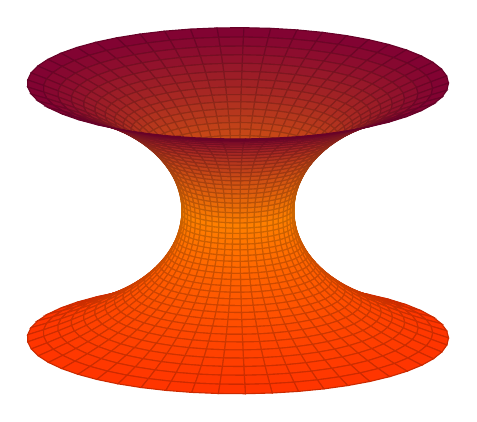
\begin{tikzpicture}
        \begin{axis}[
            view={110}{20},
            samples=\samplescalar,
            samples y=\samplescalar,
            domain=0:2*pi,
            y domain=-2:2,
            scale = 1,
            axis lines=none,
            colormap={orangered}{
                rgb(0cm)=(1,0.2,0);
                rgb(1cm)=(1,0.5,0);
                rgb(2cm)=(0.5,0,0.2);
            },
        ]
        
        % katenoida
        \addplot3[
            surf,
            z buffer=sort,
        ]
        (
            {cosh(y)*cos(deg(x))},
            {cosh(y)*sin(deg(x))},
            {y}
        );
        
        \end{axis}
    \end{tikzpicture}

    \caption{Katenoida}
\end{figure}

Za konstrukcijo katenoide izberemo holomorfno funkcijo $f(z) = \frac{1}{z^2}$ in meromorfno funkcijo $g(z) = z$ na domeni $D = \mathbb{C} \setminus \{0\}$. Ker integriramo od točke $z_0=1$ dalje, za ustrezno translacijo dodamo začetni vektor $(1,0,0)$:
\begin{align*}
    F(z) &= (1,0,0) - \Re \int_1^z \left( \frac{1}{2} \zeta^{-2} \left(1-\zeta^2\right), \, \frac{i}{2} \zeta^{-2} \left(1+\zeta^2\right), \, \zeta^{-2} \cdot \zeta \right) \, \mathrm{d}\zeta \\    
    &= (1,0,0) - \Re \int_1^z \left( \frac{1}{2}\left(\zeta^{-2}-1\right), \, \frac{i}{2}\left(\zeta^{-2}+1\right), \, \frac{1}{\zeta} \right) \, \mathrm{d}\zeta.    
\end{align*}
Prva komponenta:
\begin{align*}
    F_1 &= 1 - \Re \int_1^z \frac{1}{2}\left(\zeta^{-2}-1\right) \,\mathrm{d}\zeta \\
    &= 1 - \Re \left[ \frac{1}{2}\left(-\zeta^{-1}-\zeta\right) \right]_1^z \\
    &= 1 + \frac{1}{2} \Re \left( z + \frac{1}{z} - 2 \right) \\
    &= \frac{1}{2} \Re \left( z + \frac{1}{z} \right).
\end{align*}
S spremembo kompleksne spremenljivke $z = e^w = e^{u+\mathfrak{i}v} = r e^{\mathfrak{i}\theta}$ (kjer je $u = \ln r$ in $v = \theta$) in upoštevanje identitete $e^{\mathfrak{i} \theta}=\cos \theta+\mathfrak{i} \sin \theta$ dobimo:
\begin{equation*}
    F_1 = \frac{1}{2} \Re \left( r e^{\mathfrak{i}\theta} + \frac{1}{r} e^{-\mathfrak{i}\theta} \right) = \frac{1}{2}\left(r + \frac{1}{r}\right) \cos \theta = \cosh (\ln r) \cos \theta.
\end{equation*}
Druga komponenta:
\begin{align*}
    F_2 &= 0 - \Re \int_1^z \frac{\mathfrak{i}}{2}\left(\zeta^{-2}+1\right) \, \mathrm{d}\zeta \\
    &= -\Re \left[ \frac{\mathfrak{i}}{2}\left(-\zeta^{-1}+\zeta\right) \right]_1^z \\
    &= \frac{1}{2} \Re \left( \mathfrak{i}\left(z - \frac{1}{z}\right) \right).
\end{align*}
Na enak način kot zgoraj dobimo:
\begin{align*}
    F_2 &= \frac{1}{2} \Re \left( \mathfrak{i} \left( r(\cos \theta + \mathfrak{i} \sin \theta) - \frac{1}{r}(\cos \theta - \mathfrak{i} \sin \theta) \right) \right) \\
    &= \frac{1}{2}\left(r + \frac{1}{r}\right) \sin \theta \\
    &= \cosh (\ln r) \sin \theta.
\end{align*}
Tretja komponenta:
\begin{equation*}
F_3 = 0 - \Re \int_1^z \frac{1}{\zeta} \, \mathrm{d}\zeta = -\Re[\ln \zeta]_1^z = -\Re(\ln |z| + \mathfrak{i} \arg z) = -\ln |z| = -\ln r.
\end{equation*}
Če to prevedemo nazaj na koordinate $u$ in $v$, vidimo, da dobimo ravno začetno parametrizacijo katenoida. Torej: 
\begin{equation*}
    F(u, v) = (\cosh u \cos v, \cosh u \sin v, -u).
\end{equation*}


\subsection{Helikoid}

Helikoid sta prva opisala Leonhard Euler (1774) in Jean Baptiste Meusnier (1776). Geometrijsko ga dobimo tako, da premico v $\mathbb{R}^2$ vrtimo in jo hkrati dvigujemo v smeri osi vrtenja. Torej s parametrizacijo
\begin{align*}
    & x=\rho \cos (\theta), \\
    & y=\rho \sin (\theta), \\
    & z=\theta,
\end{align*}
za $\rho$ in $\theta$ od $-\infty$ do $\infty$.
Poleg ravnine je to edina minimalna ploskev, ki jo lahko predstavimo kot unijo premic. Take ploskve imenujemo \emph{premonosne ploskve}.

\begin{figure}[ht]
    \centering
    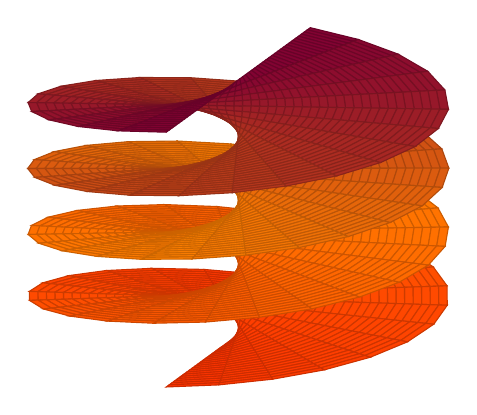
\begin{tikzpicture}
        \begin{axis}[
            view={110}{20},
            samples=\samplescalar,
            samples y=\samplescalar,
            domain=-2:2,
            y domain=0:4*pi,
            scale = 1,
            axis lines=none,
            colormap={orangered}{
                rgb(0cm)=(1,0.2,0);
                rgb(1cm)=(1,0.5,0);
                rgb(2cm)=(0.5,0,0.2);
            },
        ]
        
        % helikoid
        \addplot3[
            surf,
            z buffer=sort,
        ]
        (
            {x * cos(deg(y))}, 
            {x * sin(deg(y))}, 
            {y} 
        );
        
        \end{axis}
    \end{tikzpicture}

    \caption{Helikoid}
\end{figure}

Izberimo holomorfno funkcijo $f(z)=e^{-\mathfrak{i} z}$ in meromorfno funkcijo $g(z)=e^{\mathfrak{i} z}$. Weierstrass-Enneperjeva reprezentacija v kompleksni koordinati $z=u+\mathfrak{i} v \in \mathbb{C}$ ima obliko
\begin{align*}
    F(z)&=\Re \int_0^z\left(\frac{1}{2} e^{-\mathfrak{i} \zeta}\left(1-e^{2 \mathfrak{i} \zeta}\right), \frac{\mathfrak{i}}{2} e^{-\mathfrak{i} \zeta}\left(1+e^{2 \mathfrak{i} \zeta}\right), e^{-\mathfrak{i} \zeta} e^{\mathfrak{i} \zeta} \right) \, \mathrm{d} \zeta \\   
    &=\Re \int_0^z(-\mathfrak{i} \sin \zeta, \mathfrak{i} \cos \zeta, 1) \, \mathrm{d} \zeta    
\end{align*}
Prva komponenta:
\begin{align*}
    F_1 & =\Re \int_0^z(-\mathfrak{i} \sin \zeta) \, \mathrm{d} \zeta \\
    & =\Re[\mathfrak{i} \cos \zeta]_0^z \\
    & =\Re(\mathfrak{i} \cos (u+\mathfrak{i} v)-\mathfrak{i}) \\
    & =\Re(\mathfrak{i}(\cos u \cosh v-\mathfrak{i} \sin u \sinh v)-\mathfrak{i}) \\
    & =\Re(\sin u \sinh v+\mathfrak{i}(\cos u \cosh v-1)) \\
    & =\sin u \cdot \sinh v .
\end{align*}
Druga komponenta:
\begin{align*}
    F_2 & =\Re \int_0^z \mathfrak{i} \cos \zeta \, \mathrm{d} \zeta \\
    & =\Re[\mathfrak{i} \sin \zeta]_0^z \\
    & =\Re(\mathfrak{i} \sin (u+\mathfrak{i} v)) \\
    & =\Re(\mathfrak{i}(\sin u \cosh v+\mathfrak{i} \cos u \sinh v)) \\
    & =\Re(-\cos u \sinh v+\mathfrak{i} \sin u \cosh v) \\
    & =-\cos u \cdot \sinh v .
\end{align*}
Tretja komponenta:
\begin{equation*}
    F_3=\Re \int_0^z 1 \, \mathrm{d} \zeta=\Re(z)=\Re(u+\mathfrak{i} v)=u.
\end{equation*}
Torej dobimo parametrizacijo 
\begin{equation*}
    F(u,v) = (\sin u \sinh v, \, -\cos u \sinh v, \, u).
\end{equation*}
Pokažimo, da ta parametrizacija določa isto ploskev kot klasična geometrijska parametrizacija. Vpeljemo spremenljivki $\theta = u$ in $\rho = -\sinh v$. Funkcija $\sinh: \mathbb{R} \rightarrow \mathbb{R}$ je bijekcija, zato spremenljivka $\rho$ zavzame vse realne vrednosti. Z vstavljanjem novih spremenljivk v $F(u,v)$ dobimo:
\begin{align*}
    x &= \sin u \sinh v = -\rho \sin \theta = \rho \cos\left(\theta + \frac{\pi}{2}\right), \\
    y &= -\cos u \sinh v = \rho \cos \theta = \rho \sin\left(\theta + \frac{\pi}{2}\right), \\
    z &= u = \theta.
\end{align*}
Če zarotiramo ploskev v $(x,y)$ ravnini za kot $\frac{\pi}{2}$ (kar ne spremeni geometrije ploskve), dobimo natanko klasično parametrizacijo helikoida:
\begin{equation*}
    (x, y, z) = (\rho \cos \theta, \, \rho \sin \theta, \, \theta).
\end{equation*}


\subsection{Enneperjeva ploskev}

Enneperjevo minimalno ploskev je leta 1868 odkril nemški matematik Alfred Enneper. Za razliko od katenoide ali helikoide Enneperjeva ploskev ne izhaja iz klasičnih geometrijskih pogojev, zato zanjo ni klasične izpeljave. Enneper jo je odkril neposredno z uporabo Weierstrass-Enneperjeve formule, kjer je za $f$ in $g$ izbral najpreprostejši netrivialni funkciji.

\begin{figure}[ht]
    \centering
    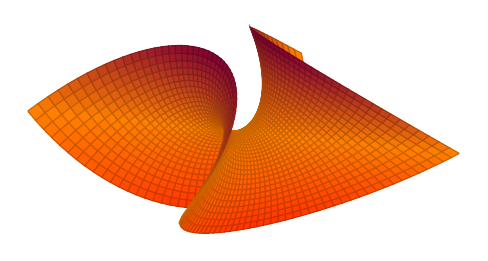
\begin{tikzpicture}
        \begin{axis}[
            view={150}{30},
            samples=\samplescalar, 
            samples y=\samplescalar,
            domain=-1.3:1.3, 
            y domain=-1.3:1.3,
            scale=0.8,
            axis lines=none,
            %colormap/viridis,
            colormap={orangered}{
                        rgb(0cm)=(1,0.2,0);
                        rgb(1cm)=(1,0.5,0);
                        rgb(2cm)=(0.5,0,0.2);
                    },
        ]
        
        % Enneperjeva ploskev 
        \addplot3[
            surf,
            z buffer = sort,
        ]
        (
            {x - (1/3) * x^3 + x * y^2}, 
            {-y - x^2 * y + (1/3) * y^3}, 
            {x^2 - y^2} 
        );
        \end{axis}
    \end{tikzpicture}
    \caption{Enneperjeva ploskev}
\end{figure}

Za holomorfno funkcijo izberemo konstanto $f(z)=2$, za meromorfno pa $g(z)=z$. Weierstrass-Enneperjeva reprezentacija se potem glasi
\begin{align*}
    F(z)&=\Re \int_0^z\left(\frac{1}{2} \cdot 2\left(1-\zeta^2\right), \frac{\mathfrak{i}}{2} \cdot 2\left(1+\zeta^2\right), 2 \zeta\right) \, \mathrm{d} \zeta \\
    & = \Re \int_0^z\left(1-\zeta^2, \mathfrak{i}\left(1+\zeta^2\right), 2 \zeta\right) \, \mathrm{d} \zeta .
\end{align*}
Prva komponenta:
\begin{align*}
    F_1 & =\Re \int_0^z\left(1-\zeta^2\right) \, \mathrm{d} \zeta=\Re\left[\zeta-\frac{\zeta^3}{3}\right]_0^z \\
    & =\Re\left((u+\mathfrak{i} v)-\frac{(u+\mathfrak{i} v)^3}{3}\right) \\
    & =\Re\left(u+\mathfrak{i} v-\frac{u^3+3 \mathfrak{i} u^2 v-3 u v^2-\mathfrak{i} v^3}{3}\right) \\
    & =u-\frac{u^3}{3}+u v^2\\
    &=u\left(1-\frac{u^2}{3}+v^2\right)
\end{align*}
Druga komponenta:
\begin{align*}
    F_2 & =\Re \int_0^z \mathfrak{i}\left(1+\zeta^2\right) \, \mathrm{d} \zeta\\
    &=\Re\left[\mathfrak{i}\left(\zeta+\frac{\zeta^3}{3}\right)\right]_0^z \\
    & =\Re\left(\mathfrak{i}\left(u+\mathfrak{i} v+\frac{u^3+3 \mathfrak{i} u^2 v-3 u v^2-\mathfrak{i} v^3}{3}\right)\right) \\
    & =\Re\left(\mathfrak{i} u-v+\frac{\mathfrak{i} u^3-3 u^2 v-3 \mathfrak{i} u v^2+v^3}{3}\right) \\
    & =-v-u^2 v+\frac{v^3}{3}\\
    &=-v\left(1+u^2-\frac{v^2}{3}\right) .
\end{align*}
Tretja komponenta:
\begin{align*}
    F_3 & =\Re \int_0^z 2 \zeta \, \mathrm{d} \zeta\\
    &=\Re\left[\zeta^2\right]_0^z \\
    & =\Re\left((u+\mathfrak{i} v)^2\right)\\
    &=\Re\left(u^2-v^2+2 \mathfrak{i} u v\right)\\
    &=u^2-v^2 .
\end{align*}
Torej dobimo parametrizacijo
\begin{equation*}
    F(u, v) = \left( u\left(1 - \frac{u^2}{3} + v^2\right), -v\left(1+u^2-\frac{v^2}{3}\right), u^2 - v^2 \right)
\end{equation*}
za $u,v \in \mathbb{R}$.

\end{document}
